\section{Principe de repondération} % Seções são adicionadas para organizar sua apresentação em blocos discretos, todas as seções e subseções são automaticamente exibidas no índice como uma visão geral da apresentação, mas NÃO são exibidas como slides separados.

%------------------------------------------------
\begin{frame}{}
	
	\huge \begin{center}
		PRINCIPE
	\end{center}
	
\end{frame}


\begin{frame}
	\frametitle{Les étapes du traitement de la non-réponse totale }
	

\vspace{0.5cm}
\begin{enumerate}
\item Identification des non-répondants,
\item Modélisation du mécanisme de non-réponse (recherche des facteurs explicatifs),
\item Estimation des probabilités de réponse,
\item Calcul des poids corrigés de la non-réponse totale.
\end{enumerate}

\end{frame}

\begin{frame}
	\frametitle{Modélisation du mécanisme de non-réponse}
	
On note $r_k$ la variable indicatrice de réponse pour l’individu k, valant
1 si l’individu a répondu à l’enquête et 0 sinon. \\ 

\[
r_k =
\begin{cases} 
	1 & \text{si l’individu $k$ a répondu}, \\
	0 & \text{sinon}.
\end{cases}
\]
\vspace{0.5cm}


On note $p_{k \mid S} \equiv p_k$ la probabilité de réponse pour l’unité $k$ : 
\[
p_k = \Pr(k \in S_r \mid S) = \Pr(r_k = 1 \mid S).
\]

\end{frame}


\begin{frame}
	\frametitle{Modélisation du mécanisme de non-réponse}

Si on veut estimer le total T d'une variable dans l'échantillon total, T est estimé sans biais par l’estimateur de \textbf{Horvitz-Thompson} : $$ \hat{T} = \sum_{k \in S} w_k y_k = \sum_{k \in S} \frac{y_k}{\pi_k}  $$

avec $w_k = \frac{1}{\pi_k}$ le poids de sondage de l’unité $k$ \\  \vspace{0.3cm}

En présence de non réponse totale, on obtient un estimateur sans biais du total T : $$\hat{T}_r =  \sum_{k \in S_r} \frac{y_k}{\pi_k \times p_k}$$
\end{frame}

\begin{frame}{}
	\begin{figure}[h]
		\centering
		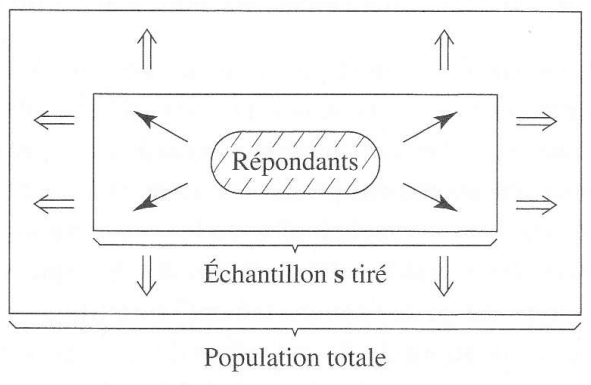
\includegraphics[width=0.9\textwidth]{img/s.png}
		%	\caption{Legenda da imagem}
		%	\label{fig:label_da_imagem}
	\end{figure}
\end{frame}

\begin{frame}
	\frametitle{Hypothèses}



On fait l’hypothèse que :
\begin{itemize}
	\item toutes les probabilités de réponse vérifient $0 < p_k \leq 1$ : pas de non-répondants irréductibles,
	\item les individus répondent indépendamment les uns des autres : 
	\[
	\Pr(k, l \in S_r \mid S) \equiv p_{kl} = p_k p_l.
	\]
\end{itemize}
Cette dernière hypothèse peut être affaiblie (Haziza et Rao, 2003 ; Skinner et D’Arrigo, 2011).


\end{frame}



\begin{frame}
	\frametitle{Types de mécanisme}

On distingue schématiquement trois types de mécanisme de non-réponse :  \\ \vspace{0.5cm}
\begin{enumerate}
	\item uniforme (ou MCAR),
	\item ignorable (ou MAR),
	\item non-ignorable (ou NMAR).
\end{enumerate}

\end{frame}


